\section{Driver Framework with Interrupts}
\label{sec:driver}

The processor inherently runs in parallel with devices. In Sec.~\ref{sec:model},
we have presented a machine model representing this level of concurrency. On top
of this machine model, we build certified abstraction layers introducing more
and more driver code. At each abstraction layer, our model enforces systematic
isolation among the different device objects and the rest of the kernel, so that
interaction with one device object does not affect the states of other device
objects nor the rest of the kernel. Thus, isolation properties are satisfied by
construction. This dramatically simplifies our reasoning by allowing us, at any
given time, to focus on only the device objects that are currently interacted
with.

In this section, we define the device object more formally; then we show how to
incorporate interrupts into our model while still following our isolation
policy.

\subsection{Device Objects}

\begin{figure}
\begin{center}
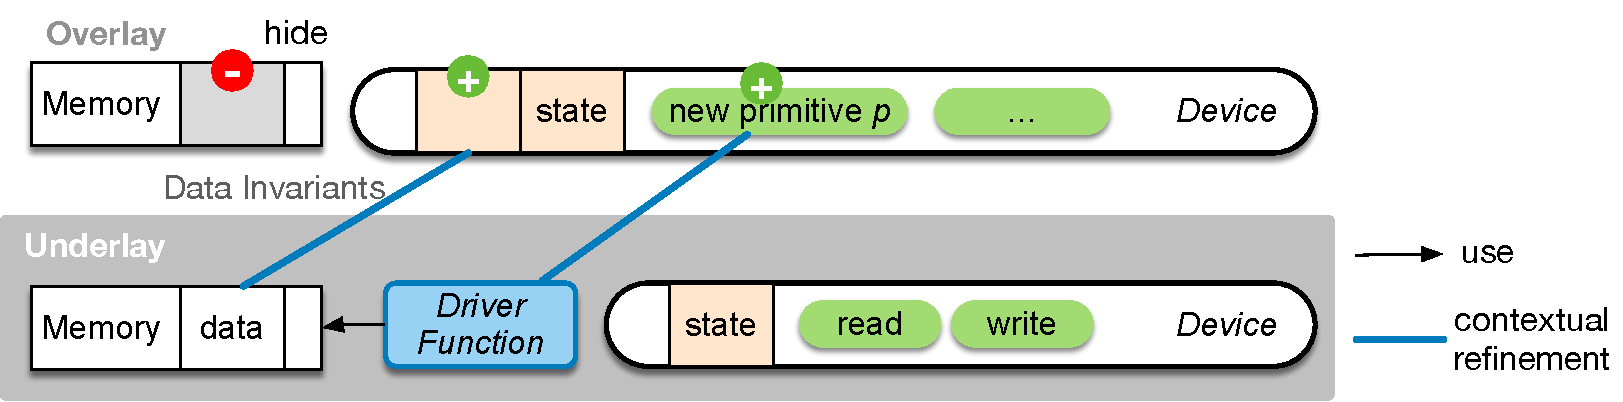
\includegraphics[width=0.95\textwidth]{figs/object}
\end{center}
\caption{Layer-based contextual refinement of the device object}
\label{fig:spec:object}
\end{figure}

\ignore{ In Chapter \ref{sec:model}, we talked about using the local and global
	log to reason about this concurrency. However, when it comes to the driver
	level, things are different. Drivers' code is executing inside CPU, but it may
	trigger device transition. Moreover, a driver usually has its own data, e.g.
	buffer, FIFO queue, which is stored in the memory. That means, while the memory
	of a driver is being changed, its device states may change at the same time. For
	example, when a driver fetching a data unit from the buffer, it may be
	interrupted by its interrupt handler, which tries to adding a unit into the
	buffer. Usually we simply disable the interrupt or mask that interrupt line
	during the fetching operation to rule out this race condition. However, we have
	to prove that the whole context, i.e. all possible program in the universe,
	disable their interrupt before touching these data. If we just mask the
	interrupt line, we have to prove all other interrupt handler in the context will
	not touch these data too. It is an impossible job. }

A {\it device object} is a logical abstraction containing a hardware device plus
its related drivers. Each device object consists of a set of abstract states,
abstracting the private states of the device (e.g., device registers, driver
private memory); and a set of primitives, abstracting the module interface. The
abstract states are private to the device object, and can only be manipulated by
explicit calls to the device object's primitives. This is achieved by
establishing a contextual refinement relation from the concrete memory and
device function implementation to the abstract state and primitives. As shown in
Fig.~\ref{fig:spec:object}, we follow the layer-based methodology introduced in
Chapter \ref{chapter:framework}
and utilize the CompCert memory permissions~\cite{leroy08} to hide the relevant
memory at overlay, which prevents the context code from accessing the object's
private data. These logical permissions do not correspond to any physical
protection mechanism but are used to ensure that the abstract machine at
overlay gets stuck if any code tries to directly access this portion of data.
The safety proof of our entire operating system (the kernel never gets stuck)
guarantees that such a situation never happens.  The set of driver functions at
underlay, which manipulates the memory that will be abstracted away at overlay,
are themselves abstracted into the set of device primitives at the overlay (see
Fig.~\ref{fig:spec:object}).

For example, the console buffer is implemented as a circular buffer in our
console driver.  The concrete implementations of the buffer operators ({\it
	cb\_read} and {\it cb\_write}) directly manipulate the concrete circular
buffer in memory. At a higher layer, in our abstract console device object, the
logical buffer is represented as a list, and the primitives are specified
directly over this abstract list, i.e., the {\it cb\_read} simply returns the
head element in the list, while {\it cb\_write} adds the new element to the end
of the list, discarding a single head element if the size of the list exceeds
its limit.  The contextual refinement relation between the two layers ensures
that any code running on top of the more abstract overlay exhibits behavior
equivalent to running on top of the underlay.

The primitives at the underlay can be passed through to the overlay, or hidden
if they are no longer needed.  For example, once the primitive {\it
	ahci\_transfer} is introduced at the overlay, the underlay primitives {\it
	ahci\_read} and {\it ahci\_write}, used to implement {\it ahci\_transfer}, are
hidden. This facilitates the invariant proofs as stronger invariants can be
introduced at higher layers, which could otherwise be violated by the
lower-level primitives.

This kind of abstraction does not necessarily have to include any code, and sometimes
are achieved already at the raw device level. For example, some part of memory
may be designated to the hardware device to set up the direct memory access (DMA)
to allow the device directly read from or write to the main memory without
going through the main CPU. In this case, the part of memory designated for DMA
can also be abstracted into the device's internal abstract states through the
contextual refinement.

\ignore{

Instead of treating a driver as part of the kernel, we treat it as an extension
of the device. As shown in Figure x \hao{need a figure}, the driver just
encapsulates the original device and includes additional functions. A driver is
the abstraction of a device, which means it is still a device, and the memory
owns by it becomes part of the internal states. Even though, the new device
still follows the rule of a general device: kernel execution and the transitions
of devices are strictly isolated, thus their reasoning can be easily separated
and composed.

If a memory block needs to be added into the internal states, we first hide it
in the memory and then add it into the volatile state of the extended device.
$s^{(+)} = (d_1: T_1, d_2: T_2, ...)$. \hao{do we need to explain more here?}
After that, we add the basic primitives to access it. In this way, the context
can only operates the data through these primitives. Moreover, only the code
belongs to this device can invoke primitives of this device. That naturally
gives the isolation of interrupt handlers between devices.

After the device becomes more abstract, we can hide the unnecessary primitives
and only expose the higher-level ones. For example, if \texttt{ahci\_transfer}
is already introduced, we will no longer need \texttt{ahci\_readl} and
\texttt{ahci\_writel}. }

\paragraph{Combining Device Objects}

At a certain abstraction layer, some drivers, or more generally, system
services, may interact with multiple device objects, by, e.g., transferring data
between two devices, or broadcasting messages to multiple devices.  At this
stage, such devices are no longer totally isolated but are synchronized through
hardware or software mechanisms.  This does not fit directly into our model
providing systematic isolation among different device objects and the rest of
the kernel.

In the above scenario, we introduce at the overlay a single heterogeneous device
object, which combines the device objects from the underlay via the newly
introduced functions. The abstract machine at overlay thereby provides
systematic isolation between the new abstract device object and the rest of the
kernel. The internal states and local logs of the combined device object are the
disjoint unions of the relevant objects at underlay, while the functions that
manipulate multiple device objects at underlay become primitives of the new
device object, operating on a wider range of internal states, at overlay. As in
all device objects, existing primitives can be either passed through to this new
device or hidden.


\subsection{Interrupts}

We now show how to adapt the interrupts into our setting.  We first present our
interrupt model at the hardware level, where the interrupt transitions are
separately defined for the CPU, the interrupt controllers (IC), and the devices.
At this low-level we lack the full behaviors of interrupt handlers, so all the
primitives verified at this machine level have the precondition that interrupts
are disabled or the corresponding interrupt lines are masked. A special flag
$\mathsf{critical}$ is defined in the abstract state of each device to make sure
that every such low-level primitive has the precondition of $\mathsf{critical}$ 
being $\mathsf{true}$ to enter the critical section for accessing the data
shared between the primitives and the interrupt handler
of the device.  On top of this hardware abstraction layer, we
incrementally introduce and verify interrupt handlers for each device through
abstraction layers.  Above a certain abstraction layer, we have full behaviors
of the interrupt handlers, so we introduce a new abstraction layer with an
abstract interrupt model, where an interrupt only changes the state of the
device object that triggered it.  This makes the interrupt completely
transparent to the CPU, the IC, and other devices; thus, guaranteeing our
desired isolation properties.  We prove the strong contextual refinement
property between these two abstraction layers to ensure that any context program
running on top of the overlay retains behavior equivalent to running atop the
underlay. Starting from the abstraction layer with the abstract interrupt model,
we support verification of any code with interrupts enabled.

%%%%%%%%%%%%%%%%%%%%%%%%%%%%%%%%%%%%%%%%%%%%%%%%%%%%%%%%%%%%%%%%%%%%%%%%%%%%
\begin{figure}[t]
	\begin{center}
		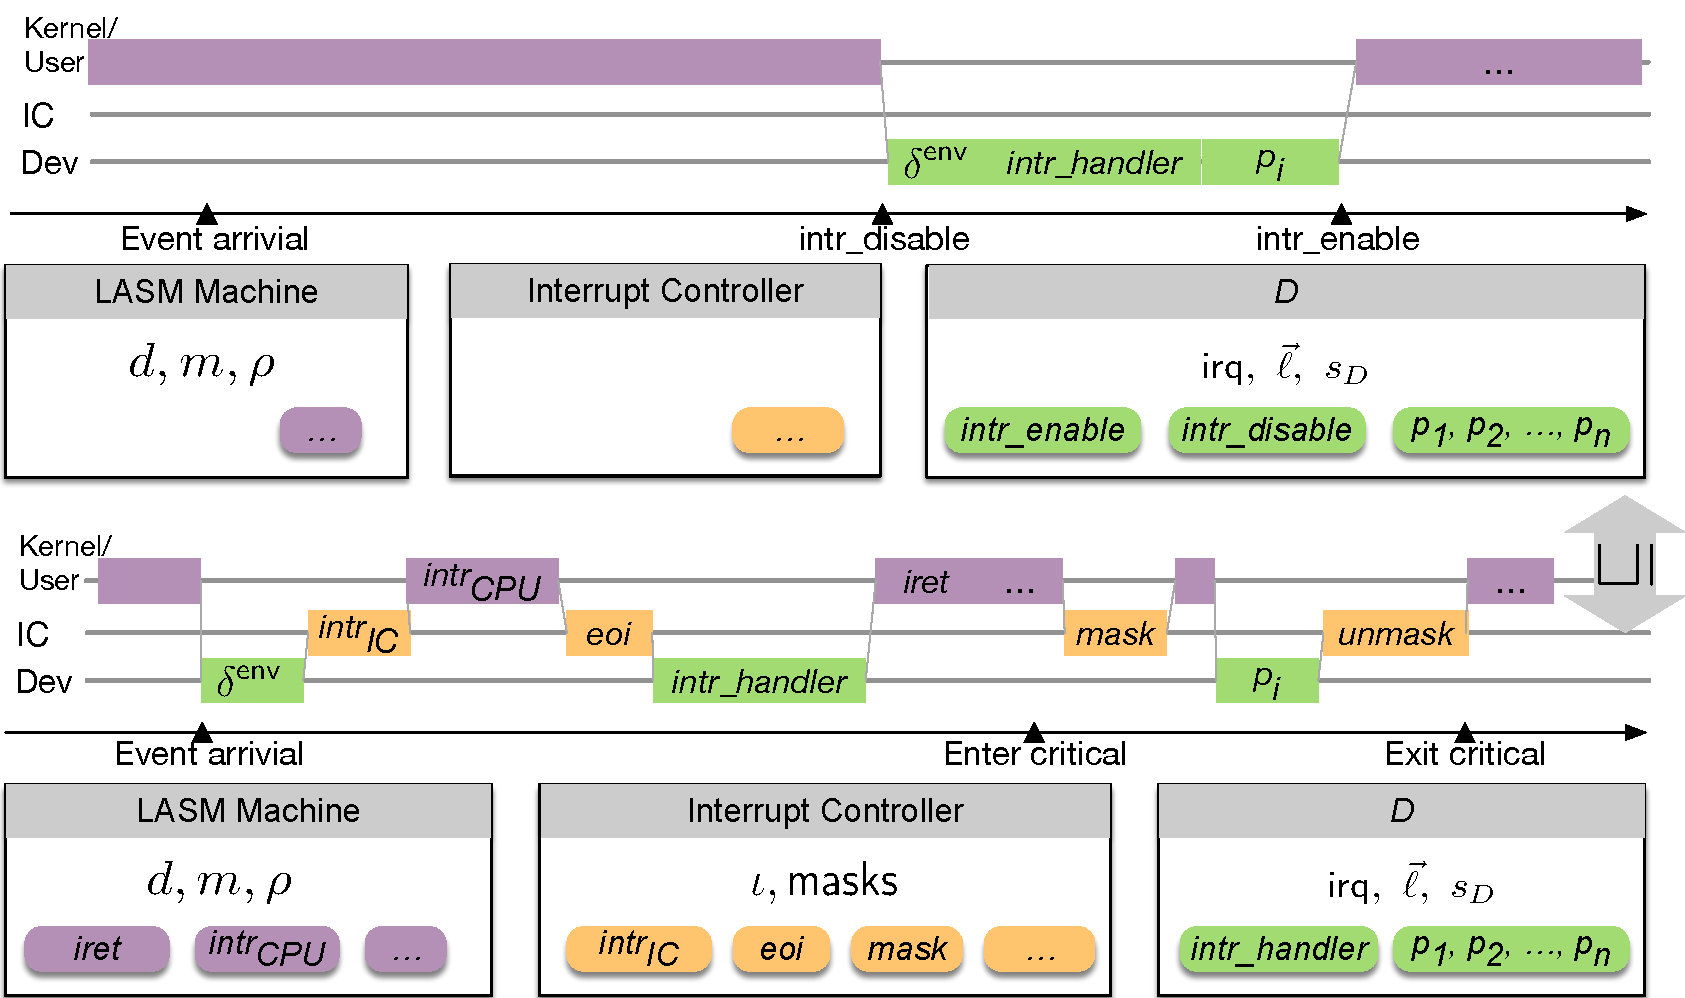
\includegraphics[scale=0.4]{figs/interrupt}
	\end{center}
	\caption{The hardware interrupt model (bottom), the
          abstract interrupt model (top), and the contextual
          refinement between these two models.}
	\label{fig:interrupt}
\end{figure}
%%%%%%%%%%%%%%%%%%%%%%%%%%%%%%%%%%%%%%%%%%%%%%%%%%%%%%%%%%%%%%%%%%%%%%%%%%%%

The entities involved in any given interrupts are categorized into three parties
(shown in the bottom half of Fig.~\ref{fig:interrupt}).  If a device transition
(e.g., from the device $D$ in Fig.~\ref{fig:interrupt}) triggers an interrupt,
it gets sent to the IC.  The IC multiplexes several interrupt lines onto the CPU
(i.e., the \textit{LAsm} machine in Fig.~\ref{fig:interrupt}), with the ability
to mask and unmask each interrupt line. At each transition, the IC selects the
pending unmasked interrupt with the highest priority and forwards it to the CPU.
When the CPU receives an interrupt signal, it first checks whether interrupts
are enabled on that CPU, and, if so, saves the current context and jumps to the
corresponding entry in the interrupt descriptor table (IDT). If interrupts are
turned off, the interrupt signal is ignored. Thus, an interrupt involves at most
three consecutive transitions: the device, the IC, and the CPU.  These three
transitions seem inter-related, and isolation among the three entities is
non-obvious.  In our approach, we first develop a low-level hardware interrupt
model that separately defines the set of interrupt-related operations.  Then
these three disconnected components are united at some higher level abstract
machine model after we have verified all the interrupt handlers.


\subsubsection{Interrupt Transition for Devices}

As described in Sec.~\ref{sec:model}, every raw device has its own
transition function $\delta^{\textsf{env}}$ specifying how it reacts
to the external events. When a particular transition triggers an
interrupt (e.g., see the event arrival and the green box
$\delta^{\textsf{env}}$ along the {\tt Dev} line in the bottom half of
Fig.~\ref{fig:interrupt}), the device marks an interrupt request bit
({\it irq}) in its internal state.


\subsubsection{Interrupt Transition for IC}
When the IC receives an interrupt signal (e.g., see the orange box
$\texttt{intr}_{\textsf{IC}}$ along the {\tt IC} line in
Fig.~\ref{fig:interrupt}), it first checks whether the particular
interrupt line is masked, and if so, it ignores the interrupt; if not,
then the IC marks the corresponding interrupt line.  The
transition rules are defined in Fig.~\ref{fig:interrupt-ic}.  Here,
$N_D$ is the corresponding interrupt line number of the device $D$
which triggered the interrupt; it is fixed by the hardware connection,
and is mapped to $\textsf{IRQ} ~ n$ by the configuration of the IC;
the $\iota$ field of $s_{\textsf{IC}}$ indicates which $\textsf{IRQ}$
number is raised; we use $\emptyset$ to indicate that there is no
raised interrupt. After the CPU performs its initial interrupt
transition, the IC would receive the End Of Interrupt (EOI) signal
(e.g., see the orange box $\texttt{eoi}$ along the {\tt IC} line in
Fig.~\ref{fig:interrupt}), it clears the raised mark on the interrupt
line.  The IC also has two primitives {\it mask} and {\it unmask},
which set the $s_{\textsf{ic}}.\textsf{masks}[N_D]$ of the interrupt
line number $N_D$ to \textsf{Masked} and \textsf{Unmasked}
respectively.


\ignore{ \hao{We do not need to extract the interrupt event. We can always let
		devices make their transition, and mark an interrupt request bit. At the
		interrupt handler level, after each transition, we check this bit. If it says
		the last transition triggered an interrupt we invoke the IC's \texttt{intr}
		primitive and check if the interrupt line is masked. If it is not, we ask CPU to
		invoke interrupt handler. When we scan the log, it indicates that the interrupt
		in the CPU is enabled. Thus, the interrupt handler will first call \texttt{eoi}
		to recover the IC. Since interrupt handler is also transparent to IC, we can
		call it in our interrupt handler. In this way, interrupt handler is a special
		device which has no local log. The reason is that every operation on it is in a
		pair (\texttt{intr}, \texttt{eoi})} }


%%%%%%%%%%%%%%%%%%%%%%%%%%%%%%%%%%%%%%%%%%%%%%%%%%%%%%%%%%%%%%%%%%%%%%%%%%%%
\begin{figure}[t]
	\begin{center}
\[
\begin{array}{cr}
	\inferrule{
			s_{\textsf{ic}}.\textsf{masks}[N_D] = \textsf{Masked} \\
			s_{\textsf{ic}}.\textsf{irqs}[N_D] = n
	}{
		\texttt{intr}_{\textsf{IC}} (s_{\textsf{ic}}, N_D) \defeq (s_{\textsf{ic}}, \emptyset) } & \text{($\texttt{intr}^{m}_{\textsf{IC}}$)} \\[5ex]

\inferrule{
		s_{\textsf{ic}}.\textsf{masks}[N_D] = \textsf{Unmasked} \\
		s_{\textsf{ic}}.\textsf{irqs}[N_D] = n \\	
		s_{\textsf{ic}}.\iota = \emptyset 
	}{
  \texttt{intr}_{\textsf{IC}} (s_{\textsf{ic}}, N_D) \defeq
           (s_{\textsf{ic}}[\iota \leftarrow \textsf{n}], \textsf{IRQ}~n)
} & \text{($\texttt{intr}^{u}_{\textsf{IC}}$)} \\[5ex]

\inferrule{
	}{	
		\texttt{eoi} (s_{\textsf{ic}}) \defeq s_{\textsf{ic}}[\iota \leftarrow \emptyset]
	} & \text{($\texttt{eoi}$)} 
\end{array}
\]
	\end{center}
	\caption{Interrupt transition for the IC}
	\label{fig:interrupt-ic}
\end{figure}
%%%%%%%%%%%%%%%%%%%%%%%%%%%%%%%%%%%%%%%%%%%%%%%%%%%%%%%%%%%%%%%%%%%%%%%%%%%%


\subsubsection{Interrupt Transition for the CPU} As soon as the IC marks 
an interrupt line as raised, the CPU will perform its own interrupt
transition (e.g., see the purple box $\texttt{intr}_{\textsf{CPU}}$
along the {\tt Kernel/User} line in Fig.~\ref{fig:interrupt}).  Let
$\rho$ represent the register set, and $d$ be the
logical abstract states in the machine model, then the interrupt
transition of a CPU is shown in Fig.~\ref{fig:interrupt-cpu}.

%%%%%%%%%%%%%%%%%%%%%%%%%%%%%%%%%%%%%%%%%%%%%%%%%%%%%%%%%%%%%%%%%%%%%%%%%%%%
\begin{figure}[t]
	\begin{center}
	\[
	\begin{array}{cr}
	\inferrule{
		\rho[\textsf{EFLAGS}.\textsf{if}] = \textsf{Disabled} 
	}{
	\texttt{intr}_{\textsf{CPU}} (d, \rho, \textsf{IRQ}~n) \defeq (d, \rho)
	} & \text{($\texttt{intr}^{d}_{\textsf{CPU}}$)} \\[5ex]

	\inferrule{
		\rho[\textsf{EFLAGS}.\textsf{if}] = \textsf{Enabled} \\
       		d' = d[\textsf{isr} \leftarrow \textsf{true}] \\
		\textsf{tfs'} = \texttt{save\_context}(d'[\textsf{tfs}], \rho)\\\\
		d'' = d'[\textsf{tfs} \leftarrow \textsf{tfs'}] \\
                		\textsf{IDT}[n] = p \\
		\rho' = \rho[\textsf{EIP} \leftarrow p][\textsf{EFLAGS}.\textsf{if} \leftarrow \textsf{Disabled}]
	}{
	\texttt{intr}_{\textsf{CPU}} (d, \rho, \textsf{IRQ}~n) \defeq (d'', \rho') 
	} & \text{($\texttt{intr}^{e}_{\textsf{CPU}}$)}  \\[5ex]

	\inferrule{
		(\textsf{tfs'}, \rho') = \texttt{restore\_context}(d[\textsf{tfs}]) \\
		d' = d[\textsf{isr} \leftarrow \textsf{false}][\textsf{tfs} \leftarrow \textsf{tfs'}]
	}{
	\texttt{iret} (d, \rho) \defeq (d', \rho') 
} & \text{($\texttt{iret}$)} 
\end{array}
\]
	\end{center}
	\caption{Interrupt transition for the CPU}
	\label{fig:interrupt-cpu}
\end{figure}
%%%%%%%%%%%%%%%%%%%%%%%%%%%%%%%%%%%%%%%%%%%%%%%%%%%%%%%%%%%%%%%%%%%%%%%%%%%%

We use $\textsf{EFLAGS.if}$ to represent the interrupt flag
bit in the $\textsf{EFLAGS}$ register.  If interrupts are disabled
inside the CPU, the $\texttt{intr}_{\textsf{CPU}}$ primitive is totally
transparent. Otherwise, it first changes the logical \texttt{isr}
state to \texttt{true}, saves the current context into the end of the
trap frame list ($d'[\texttt{tfs}]$), and jumps to the corresponding IDT
entry. Here \texttt{isr} indicates whether the current machine
execution is in the interrupt handling mode; the \texttt{save\_context}
function models the hardware behavior of saving the current context into
the abstract state ($d'[\texttt{tfs}]$), which corresponds to the concrete
stack frames in the memory (abstracted in layers below). 

The primitive \texttt{iret} is the counterpart of
$\texttt{intr}_{\textsf{CPU}}$, and models the behavior of CPU when
the interrupt handler returns.  It restores $\textsf{EFLAGS}$
(including the old interrupt flag bit) from the context and thus also
re-enable interrupts. The \texttt{restore\_context} function
models the hardware behavior of restoring the current context
from the abstract state ($d[\texttt{tfs}]$).

\begin{lemma} \label{lemma:context}
  The function \texttt{restore\_context} is a left inverse of
  the function \texttt{save\_context}. 
  
  \[\begin{array}{c}
		\inferrule{
			\textsf{tfs}' = \texttt{save\_context}(d[\textsf{tfs}], \rho) \\\\ 
			(d', m', \rho') = f (d[\textsf{tfs}\leftarrow\textsf{tfs}'], m, \rho) \\\\
			d[\textsf{tfs}] = d'[\textsf{tfs}] \\\
			(\textsf{tfs}'', \rho'') = \textsf{restore\_context}(d'[\textsf{tfs}])
		}{
			\textsf{tfs} = \textsf{tfs}'' \wedge \rho = \rho '' 
		} 
  \end{array}\]
  
  \ignore{
  $(\texttt{tfs}, \rho) = \textsf{restore\_context}(\texttt{save\_context}(\textsf{tfs}, \rho))$
  }
\end{lemma}

The CPU also has two primitives {\it sti} and {\it cli}, which
set the $\textsf{EFLAGS}.\textsf{if}$ bit to \textsf{Enabled}
and \textsf{Disabled} respectively.

% In the bottom half of Figure~\ref{fig:interrupt}


%%%%%%%%%%%%%%%%%%%%%%%%%%%%%%%%%%%%%%%%%%%%%%%%%%%%%%%%%%%%%%%%%%%%%%%%%%%%
\begin{figure}[t]
	\[\begin{array}{lc}
\multicolumn{2}{l}{\textsc{DisableNoIntr:} ~ \text{Disable with no unhandled interrupt}} \\[1ex]
& \inferrule{
		(e, \ell'_i) = \textsf{next} (\ell^{env}, \ell_i) \\	
		s_{\textsf{tmp}} = \delta^{\textsf{env}} (s, e) \\\\
		s_{\textsf{tmp}}.irq = \textsf{false} \\
		s' = s[\textsf{critical} \leftarrow \textsf{true}] 
	}{
	\texttt{intr\_disable} (s, \ell_i, \ell^{env}) \defeq (s', \ell_i) 
} \\[5ex]

\multicolumn{2}{l}{\textsc{DisableIntr:} ~ \text{Disable with unhandled interrupts}} \\[1ex]
& \inferrule{
		(e,\ell'_i) = \textsf{next} (\ell^{env}, \ell_i) \\	
		s' = \delta^{\textsf{env}} (s, e) \\\\
		s'.irq = \textsf{true} \\
		(s'', \ell_i'') = \texttt{intr\_handler} (s', \ell'_i, \ell^{env}) \\
		(s''', \ell_i''') = \texttt{intr\_disable} (s'', \ell''_i, \ell^{env}) 
	}{
	\texttt{intr\_disable} (s, \ell_i, \ell^{env}) \defeq (s''', \ell_i''') 
} \\[5ex]

\multicolumn{2}{l}{\textsc{EnableNoIntr:}~\text{Enable with no raised interrupt}}\\[1ex]
& \inferrule{
	s.irq = \textsf{false} \\
	s' = s[\textsf{critical} \leftarrow \textsf{false}] 
}{
\texttt{intr\_enable} (s, \ell_i, \ell^{env}) \defeq (s', \ell_i) 
}\\[5ex]

\multicolumn{2}{l}{\textsc{EnableIntr:} ~ \text{Enable with raised interrupts}}\\[1ex]
& \inferrule{
	s.irq = \textsf{true} \\
	(s', \ell'_i) = \texttt{intr\_handler} (s, \ell_i, \ell^{env}) \\
	(s'', \ell_i'') = \texttt{intr\_enable}(s', \ell_i', \ell^{env}) 
}{
	\texttt{intr\_enable} (s, \ell_i, \ell^{env}) \defeq (s'', \ell_i'') 
}
\end{array}\]
\caption{Transition rules for {\it intr\_disable} and {\it intr\_enable}}
	\label{fig:intr-transition}
\end{figure}

%%%%%%%%%%%%%%%%%%%%%%%%%%%%%%%%%%%%%%%%%%%%%%%%%%%%%%%%%%%%%%%%%%%%%%%%%%%%

\subsubsection{Abstract Interrupt Model} \label{sec:interrupt}

The low-level machine model, we just described, is not suitable for
reasoning about interrupts, since each of the three entities has its
own disconnected view.  For instance, when the CPU jumps to an IDT
entry, it is unaware of the behavior of the corresponding interrupt
handler, and when the IC sends an interrupt signal to the CPU, it does
not know whether the interrupt will be handled or not. We would like
to formally connect these three different views to derive a nice
machine model that is suitable for reasoning about the end-to-end
behavior of interrupts, i.e., an interrupt triggered by a device only
modifies the particular device's internal states, and is transparent
to the CPU, the IC, and other devices.  To achieve this, we need a
model of the full behavior of the interrupt handler for each device.

Starting from the above hardware interrupt model, we incrementally extend a raw
device by wrapping it with driver code related to the interrupt handler, until
we have fully verified the interrupt handler for the device.  Each device has
exactly one interrupt handler, which, by our isolation policy, only modifies
the internal states of its particular device (Lemma~\ref{lemma:intr-handler}),
and cannot itself be interrupted by the same device.

\begin{lemma} \label{lemma:intr-handler}
The interrupt handler (\texttt{intr\_handler}) of device $D$ can only observe
and modify the abstract states of $D$.
%\[
%\begin{array}{c}
%	\inferrule{
%		d = (s_1, s_2, ..., s_D, ...) \\
%		d' = (s'_1, s'_2, ..., s'_D, ...) \\
%		s_D = s'_D \\
%	}{
%		\texttt{intr\_handler}_D (d, \ell_i, \ell^{env}) \defeq \texttt{intr\_handler}_D (d', \ell_i, \ell^{env}) 
%	}\\[5ex]
%	\inferrule{
%		d = (s_1, s_2, ..., s_D, ...) \\
%		d' = (s'_1, s'_2, ..., s'_D, ...) \\
%		(d, \ell'_i) = \texttt{intr\_handler}_D (d, \ell_i, \ell^{env}) \\
%		1 \le j \le |d| \\
%		j \neq D
%	}{
%		 s_j = s'_j \\
%	}
%	\end{array}
%\]
\end{lemma}

At this stage, we have the formal specification of the interrupt
handler for a device.  Next, through contextual refinement, we
encapsulate the behaviors of interrupts into two primitives {\it
  intr\_enable} and {\it intr\_disable} at overlay for the device,
which, as shown in the top half of Fig.~\ref{fig:interrupt}, render
interrupts transparent to the CPU and the IC.  The precise
transition rules are given in Fig.~\ref{fig:intr-transition}. 
Here, the $\textsf{next}$
function, as defined at the end of Sec.~\ref{sec:model}, returns the
next relevant event in $\ell^{env}$ and a new local log synchronized
with $\ell^{env}$ up to the returned event. Before,
the states on whether each device's interrupt line is masked or not
were part of the IC devices. Following our isolation policy, in the
new abstract interrupt model, we introduce a new abstract state
$\textsf{critical}$ in the device itself to indicate whether the particular
interrupt is masked. When $\textsf{critical}$ is $\textsf{true}$,
it indicates that the interrupt line for the device is masked, thus
the execution can enter the critical sections to read and write the device
internal states, and {\it vice versa}. Recall that all the low-level
primitives (ones introduced before the interrupt handler) of the device
have the precondition of $\textsf{critical}$ to be 
$\textsf{true}$ to enter the critical section.

The {\it intr\_disable} primitive first synchronizes the device state
with the previously unhandled interrupts then sets interrupt as
disabled.  It performs the synchronization by scanning the log from
the last place {\it intr\_enable} was called until we hit the first
event that did not trigger an interrupt.  This ensures that
subsequent observations on the device (in the abstract model) will be
consistent with those performed under the hardware interrupt model.
Note that {\it intr\_disable} is defined recursively: it performs the
environment transition $\delta^{\textsf{env}}$ on each event until we
hit an event that does not trigger interrupts (i.e., the
\textsc{DisableNoIntr} case); the $s_{\textsf{tmp}}$ state should be 
discarded since the device
transition stops at the point where the last unhandled interrupt is
handled.

The {\it intr\_enable} primitive discharges any raised interrupts
then sets interrupt as enabled. This models the physical machine
behavior, wherein interrupts (which can occur while interrupts are
disabled) get delayed until interrupts are re-enabled. This causes the
OS to immediately jump to the interrupt handler after re-enabling
interrupts. This repeats until the device no longer attempts to
trigger an interrupt within the interrupt handler, and normal
execution can continue.

With these two new primitives, the CPU transition in the abstract
interrupt model can be completely oblivious of the device
transitions. For example, in the top half of Fig.~\ref{fig:interrupt},
the purple box along the {\tt Kernel/User} line can ignore any event
arrival from a device; the CPU for the {\tt Kernel/User} line would
only force the device transitions when it wants to make observations
about a device (e.g., by calling {\it intr\_disable}, then a
high-level device primitive $p_i$, followed by {\it intr\_enable}).


\ignore{ Fig.~\ref{fig:intr_enable}(a) shows an example behavior of
  {\it intr\_disable} primitive at the overlay.  During a period in
  which the CPU performs a sequence of actions that are unrelated to a
  device, said device may have performed interrupt-triggering
  transitions related to the current local log, and the interrupts
  triggered during this period were immediately handled by the CPU.
  Then before calling any low-level device primitives, we first need
  to turn off the interrupt (through {\it intr\_disable}), since those
  primitives were introduced at abstraction layers lower than the
  underlay in Fig.~\ref{fig:interrupt}, which assume the interrupt
  is turned off.  Since at overlay the effects of an interrupt can
  only be observed after {\it intr\_disable} is called, we can hold
  {\it intr\_disable} responsible for ``playing'' all the related
  device transitions and interrupts that occurred since the last {\it
    intr\_enable}. Thus {\it intr\_disable} is responsible for
  synchronizing the device object's internal state with the
  transitions of both the device and interrupt handler (see Fig.~\ref{fig:intr_enable}(a)).

Fig.~\ref{fig:intr_enable}(b) illustrates an example scenario of
{\it intr\_enable}. On the actual hardware, when the interrupt is
disabled, the interrupt triggered by the device's environmental
transitions are ignored by the CPU. On the other hand, the interrupt
signal of particular interrupt line of the device remains active in
the IC, and the interrupt immediately gets handled when the interrupt
is enabled.  Note that the interrupt handler is not interruptible.
During the interrupt handling phase, more external events may trigger
interrupt, which immediately gets handled once the interrupt handler
returns back to the CPU. Thus, at the overlay, {\it intr\_enable} is
responsible for ``playing'' all of these interrupt handling
transitions (see Fig.~\ref{fig:intr_enable}(b)).

\begin{figure}
\begin{center}
	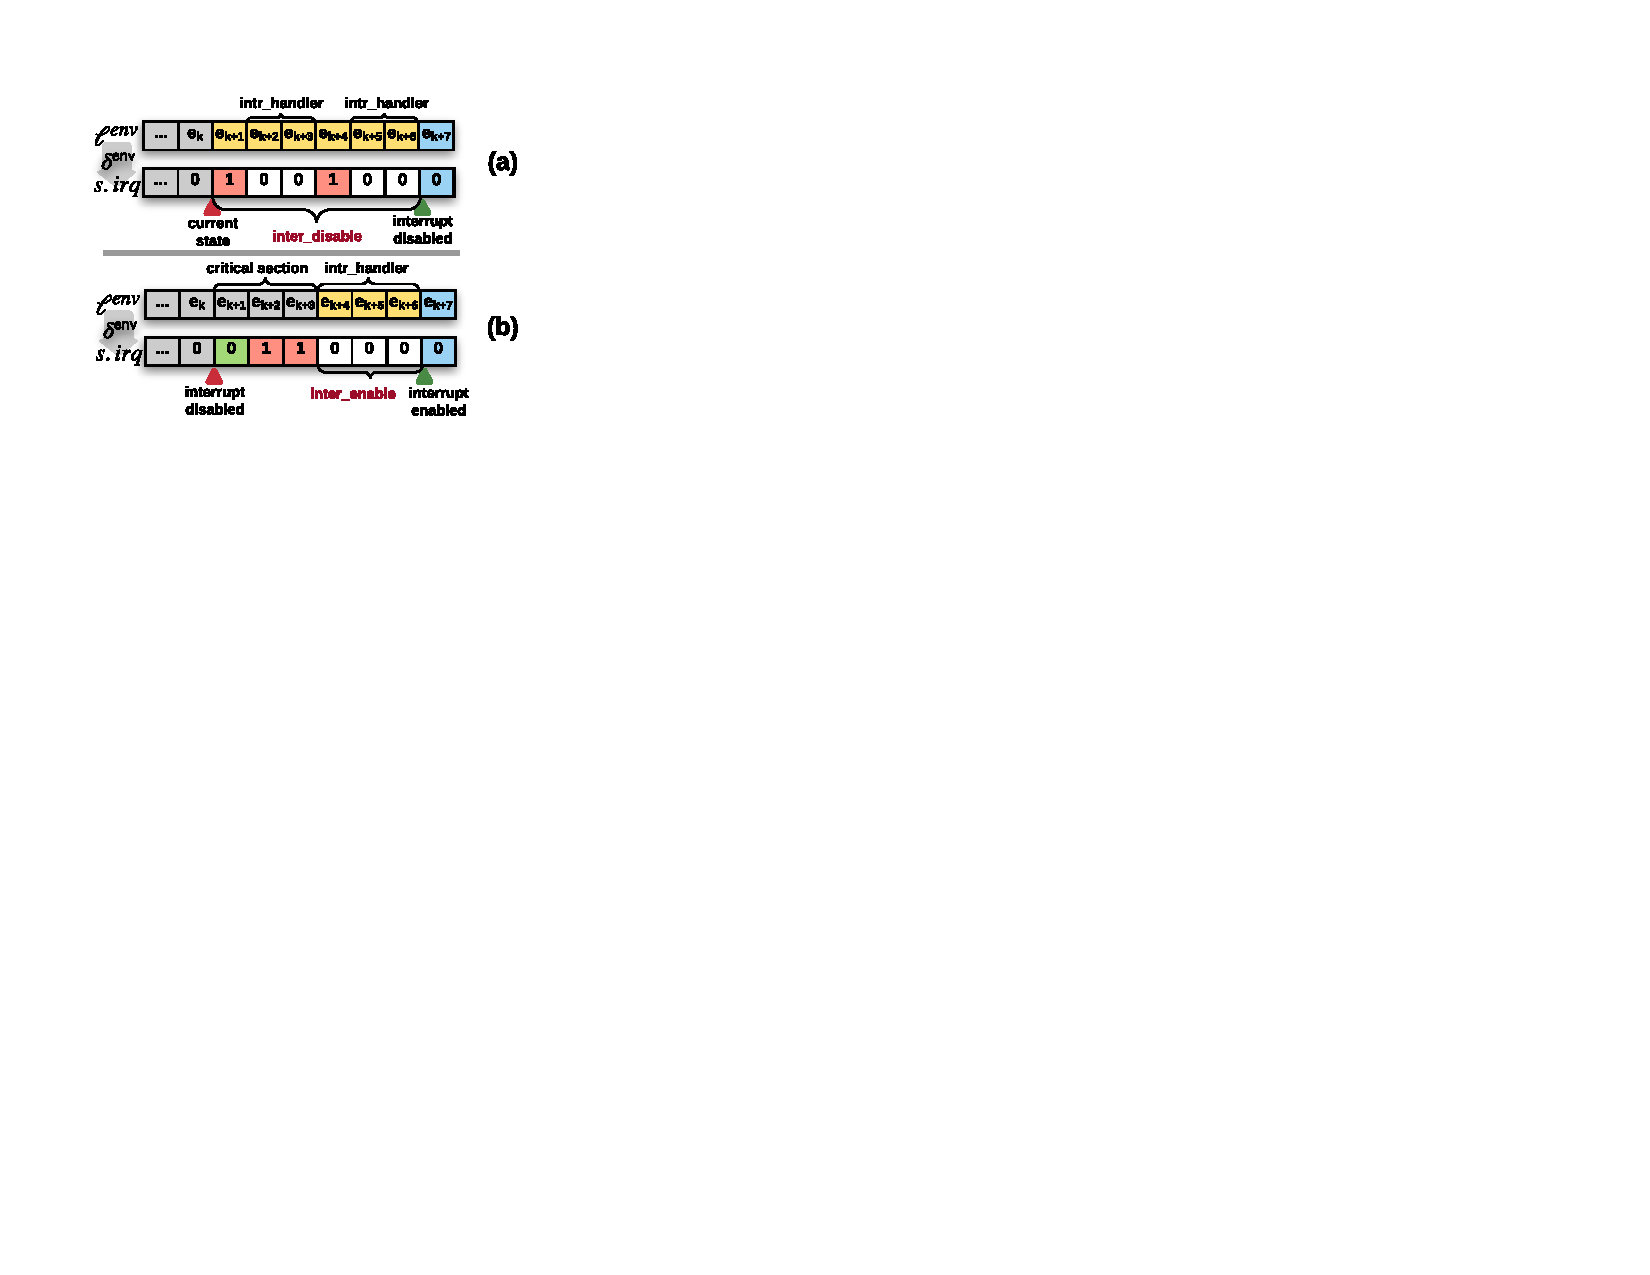
\includegraphics[scale=0.95]{figs/intr_enable}
\end{center}
\caption{Example behaviors of \texttt{intr\_disable} and \texttt{intr\_enable}.}
\label{fig:intr_enable}
\end{figure}
}




\ignore{
\paragraph{Contextual Refinement Between Two Interrupt Models} We uses several
steps to prove the contextual refinement between the two abstraction layers in
Fig.~\ref{fig:interrupt}. The goal of the refinement can be formalized as: for
device $D$ and a code fragment $f$ which ends with an primitive to disable /
enable interrupt of $D$, execution of that code on a hardware interrupt machine
is contextually equivalent to performing the same action on the abstract
interrupt machine. That is,
\[
\begin{array}{c}
\inferrule{
	(s_{hw}, m_{\mathsf{hw}}, \rho_{\mathsf{hw}}, s_{\textsf{IC\_hw}}, s_{D\_{\mathsf{hw}}}) \le_{R} (s_{abs}, m_{\mathsf{abs}}, \rho_{\mathsf{abs}}, s_{\textsf{IC\_abs}}, s_{D\_{\mathsf{abs}}}) \\
	(s'_{hw}, m'_{\mathsf{hw}}, \rho'_{\mathsf{hw}}, s'_{\textsf{IC\_hw}}, s'_{D\_{\mathsf{hw}}}, \ell'_i) =  \llbracket f \rrbracket_{\mathsf{hw}} (s_{hw}, m_{\mathsf{hw}}, \rho_{\mathsf{hw}}, s_{\textsf{IC\_hw}}, s_{D\_{\mathsf{hw}}}, \ell_i, \ell^{env}) \\
	(s'_{abs}, m'_{\mathsf{abs}}, \rho'_{\mathsf{abs}}, s'_{\textsf{IC\_abs}}, s'_{D\_{\mathsf{abs}}}, \ell'_i) =  \llbracket f \rrbracket_{\mathsf{abs}} (s_{abs}, m_{\mathsf{abs}}, \rho_{\mathsf{abs}}, s_{\textsf{IC\_abs}}, s_{D\_{\mathsf{abs}}}, \ell_i, \ell^{env}) \\
}{
	(s'_{hw}, m'_{\mathsf{hw}}, \rho'_{\mathsf{hw}}, s'_{\textsf{IC\_hw}}, s'_{D\_{\mathsf{hw}}}) \le_{R} (s'_{abs}, m'_{\mathsf{abs}}, \rho'_{\mathsf{abs}}, s'_{\textsf{IC\_abs}}, s'_{D\_{\mathsf{abs}}})
}
\end{array}
\]

Here, the evaluation of a code fragment takes an abstract state of kernel
$s$, the memory $m$, the register set $\rho$, the state of interrupt
controller $s_{\textsf{ic}}$, the state of the device $s_{D}$, a local log of
the device $\ell_i$, the event list $\ell^{env}$, and returns appropriate new
system states after the interrupt transition is fully performed.

Code fragment $f$ can be split into two disjoint parts: the part without the
last primitive ($f'$) and the last primitive ($p$). Let us assume that there is
no interrupt disabling and enabling for $D$ in the middle of $f'$. If there is, we can apply the same goal with that smaller fragment. The execution of $f$
in both machine is the sequential concatenation of the two parts:
\[
\inferrule {
	f = f'; p \\
	(s'_{os}, m', \rho', s'_{\textsf{IC}}, s'_{D}, \ell'_i) =  \llbracket f' \rrbracket (s_{os}, m, \rho, s_{\textsf{IC}}, s_{D}, \ell_i, \ell^{env}) \\
	(s''_{os}, m'', \rho'', s''_{\textsf{IC}}, s''_{D}, \ell''_i) =  \llbracket p \rrbracket (s'_{os}, m', \rho, s'_{\textsf{IC}}, s'_{D}, \ell'_i, \ell^{env})
} {
	(s''_{os}, m'', \rho'', s''_{\textsf{IC}}, s''_{D}, \ell''_i) =  \llbracket f \rrbracket (s_{os}, m, \rho, s_{\textsf{IC}}, s_{D}, \ell_i, \ell^{env})
}
\]

\noindent{}Case 1: $p$ is \texttt{intr\_disable}.

In the hardware interrupt machine, the execution of $\llbracket f'
\rrbracket_{\textsf{hw}}$ may interleave with interrupt transitions. To prove
the contextual refinement in this case, we first show that the result of these
transitions only change the state of the device, and then with the the isolation
policy, we show that all the interrupt transitions performed during the
execution of $f'$ equivalent to be done before \textsf{intr\_disable}.

\begin{figure}
	\begin{center}
	\[
	\begin{array}{c}
	\inferrule{
		(s'_{\textsf{ic}}, \textsf{IRQ} ~ n) = \texttt{intr}_{\textsf{IC}}(s_{\textsf{ic}}, N_D) \\\\
		(s',\rho') = \texttt{intr}_{\textsf{CPU}}(s, \rho, \textsf{IRQ} ~ n) \\\\
		s''_{\textsf{ic}} = \texttt{eoi}(s'_{\textsf{ic}}) \\
		(s'_{D}, \ell'_i) = \texttt{intr\_handler}_{\textsf{D}}(s_{D}, \ell_i, \ell^{env}) \\
		(d'', \rho'') =  \texttt{iret} (s', \rho') 
	}{
	   \texttt{intr}(s, m, \rho, s_{\textsf{ic}}, s_{D}, \ell_i, \ell^{env})
          	\defeq	(s'', m, \rho'', s''_{\textsf{ic}}, s'_{D}, \ell'_i) 
	} 
	\end{array}
	\]
	\end{center}
	\caption{Interrupt transition for the whole system, in the case when an
	interrupt is triggered by the device $D$ on interrupt line number $N_D$. 
		}
	\label{fig:int-whole-system}
\end{figure}

\begin{lemma}\label{lemma:irq}
	An IRQ is transparent to the CPU and the IC, i.e., the transitions triggered
	by the IRQ only change the states of the corresponding device that triggered the interrupt.
\end{lemma}
\noindent{}\begin{myproof}
	When the interrupt is disabled on the CPU or the particular interrupt line is
masked in the IC, the proof is obvious. When the interrupt is enabled, i.e.,
the corresponding interrupt line is routed, not masked, and the
\textsf{EFLAGS.if} register bit is set, the state transition of the whole
system is shown in Fig.~\ref{fig:int-whole-system}.   In this case, we need to show that:
\[\begin{array}{c}
		\inferrule{
			(s', m', \rho', s'_{\textsf{ic}}, s'_{D}, \ell'_{i}) 
			= \texttt{intr}(s, m, \rho, s_{\textsf{ic}}, s_{D}, \ell_{i}, \ell^{env}) 
		}{
			(s'_{D}, \ell'_{i}) = \texttt{intr\_handler}_{\textsf{D}}(s_{D}, \ell_{i}, \ell^{env}) \wedge \\
			 s' = s \wedge m' = m \wedge \rho' = \rho \wedge s'_{\textsf{ic}} = s_{\textsf{ic}} 
		} 
  \end{array}\]
\noindent{}This can be proven by composing the interrupt transition
rules of the CPU and the IC with Lemma \ref{lemma:context} and Lemma \ref{lemma:intr-handler}.
\end{myproof}

\begin{corollary} \label{corollary:irq}
IRQs do not affect the kernel, i.e., they do not change any of the
kernel's states\footnote{Remember, we consider device drivers a part
  of the device, not the kernel.}.
\ignore{
More formally, let the predicate $\texttt{kernel\_states} ~s$ represent a record containing
all the kernel states in the global system state $s$, then
\[\begin{array}{c}
		\inferrule{
			\texttt{intr\_handler}(s) = s' \\
		}{
			\texttt{kernel\_states} ~s = \texttt{kernel\_states} ~s' \\
		} \\
		\end{array}
		\]
}
\end{corollary}

\begin{lemma}
The execution of $\llbracket f' \rrbracket$ in both machine will have the same
result of kernel abstract state $s$, memory $m$, register set $\rho$ and the
state of interrupt controller $s_{\textsf{IC}}$. That is,
\[
\inferrule{
	(s_{hw}, m_{\mathsf{hw}}, \rho_{\mathsf{hw}}, s_{\textsf{IC\_hw}}, s_{D\_{\mathsf{hw}}}) \le_{R} (s_{abs}, m_{\mathsf{abs}}, \rho_{\mathsf{abs}}, s_{\textsf{IC\_abs}}, s_{D\_{\mathsf{abs}}}) \\
	(s''_{hw}, m''_{\mathsf{hw}}, \rho''_{\mathsf{hw}}, s''_{\textsf{IC\_hw}}, s''_{D\_{\mathsf{hw}}}, \ell''_i) =  \llbracket f' \rrbracket_{\mathsf{hw}} (s_{hw}, m_{\mathsf{hw}}, \rho_{\mathsf{hw}}, s_{\textsf{IC\_hw}}, s_{D\_{\mathsf{hw}}}, \ell_i, \ell^{env}) \\
	(s''_{abs}, m''_{\mathsf{abs}}, \rho''_{\mathsf{abs}}, s''_{\textsf{IC\_abs}}, s''_{D\_{\mathsf{abs}}}, \ell''_i) =  \llbracket f' \rrbracket_{\mathsf{abs}} (s_{abs}, m_{\mathsf{abs}}, \rho_{\mathsf{abs}}, s_{\textsf{IC\_abs}}, s_{D\_{\mathsf{abs}}}, \ell_i, \ell^{env}) \\
}{
	s''_{hw} \le_{R} s''_{abs} \\
	m''_{hw} \le_{R} m''_{abs} \\
	\rho''_{hw} \le_{R} \rho''_{abs} \\
	s''_{\textsf{IC\_hw}} \le_{R} s''_{\textsf{IC\_hw}} \\
}
\]
\end{lemma}

\noindent{}\begin{myproof}
From the Corollary~\ref{corollary:irq}, the interrupt transitions only change
the state of devices. Thus, even there is interleaving in the execution of
$\llbracket f' \rrbracket_{hw}$, it will not affect the transition of kernel and
IC.
\end{myproof}

\begin{lemma}
	After executes the same number of $\texttt{intr\_handler}_D$ in the abstract
interrupt machine at the end of $\llbracket f' \rrbracket_{abs}$, the device
state will be the same as the hardware interrupt one. The number depends on $\ell^{env}$.
	\[
	\inferrule{
		(s_{hw}, m_{\mathsf{hw}}, \rho_{\mathsf{hw}}, s_{\textsf{IC\_hw}}, s_{D\_{\mathsf{hw}}}) \le_{R} (s_{abs}, m_{\mathsf{abs}}, \rho_{\mathsf{abs}}, s_{\textsf{IC\_abs}}, s_{D\_{\mathsf{abs}}}) \\
		(s''_{hw}, m''_{\mathsf{hw}}, \rho''_{\mathsf{hw}}, s''_{\textsf{IC\_hw}}, s''_{D\_{\mathsf{hw}}}, \ell''_i) =  \llbracket f' \rrbracket_{\mathsf{hw}} (s_{hw}, m_{\mathsf{hw}}, \rho_{\mathsf{hw}}, s_{\textsf{IC\_hw}}, s_{D\_{\mathsf{hw}}}, \ell_i, \ell^{env}) \\
		(s''_{abs}, m''_{\mathsf{abs}}, \rho''_{\mathsf{abs}}, s''_{\textsf{IC\_abs}}, s''_{D\_{\mathsf{abs}}}, \ell_i) =  \llbracket f' \rrbracket_{\mathsf{abs}} (s_{abs}, m_{\mathsf{abs}}, \rho_{\mathsf{abs}}, s_{\textsf{IC\_abs}}, s_{D\_{\mathsf{abs}}}, \ell_i, \ell^{env}) \\
		(s'''_{D\_{\mathsf{abs}}}, \ell'''_i) = \texttt{intr\_handler\_next} (s''_{D\_{\mathsf{abs}}}, \ell''_i, \ell^{env}) 
		}{
		s'''_{D\_{\mathsf{abs}}} \le_{R} s''_{D\_{\mathsf{hw}}}
	}
	\],
\noindent{}where \texttt{intr\_handler\_next} is defined as:
\[
\inferrule{
	(e,\ell'_i) = \textsf{next} (\ell^{env}, \ell_i) \\	
	s' = \delta^{\textsf{env}} (s, e) \\
	s'.irq = \textsf{true} \\
	(s'', \ell_i'') = \texttt{intr\_handler} (s', \ell'_i, \ell^{env}) \\
	(s''', \ell_i''') = \texttt{intr\_handler\_next} (s'', \ell''_i, \ell^{env}) \\
}{
	\texttt{intr\_handler\_next} (s, \ell_i, \ell^{env}) \defeq (s''', \ell_i''') 
}
\]
\[
\inferrule{
	(e,\ell'_i) = \textsf{next} (\ell^{env}, \ell_i) \\	
	s' = \delta^{\textsf{env}} (s, e) \\
	s'.irq = \textsf{false} \\
}{
	\texttt{intr\_handler\_next} (s, \ell_i, \ell^{env}) \defeq (s, \ell_i) 
}
\]
\end{lemma}

\noindent{}\begin{myproof}
From the Lemma~\ref{lemma:intr-handler}, the interrupt transitions do not depend
on the state of kernel and other devices, so the result of the interrupt handler
is location independent.
\end{myproof}

\begin{lemma}
	The execution of the interrupt disabling in both machine keeps the refinement
relation.
\end{lemma}
\noindent{}\begin{myproof}
In the hardware interrupt model, we use $\texttt{mask}~n$ to disable the
interrupt for a certain device. This $n$ is unique and the mask bit of $n$ is
mapped to the $\textsf{critical}$ flag in the abstract level. When the interrupt
line is masked, $\textsf{critical} = \textsf{true}$, and otherwise
$\textsf{critical} = \textsf{false}$. This relation is proved by its definition.
\end{myproof}

\noindent{}Case 2: $p$ is \texttt{intr\_enable}.

This means the interrupt is disabled in the $f'$. It is true that we can also
call \texttt{intr\_enable} when the interrupt is enabled. However, the semantics
of this equivalent to \textsf{nop}. Thus, we forbid calling interrupt disable /
enable function that is not paired.

\begin{lemma}
	The execution of $\llbracket f' \rrbracket$ is the same for both machine when the interrupt is disabled.
\end{lemma}
\noindent{}\begin{myproof}
If the interrupt is disabled, there is no interleaving of $f'$ and interrupt
handler. The device will set its \textsf{irq} state to \textsf{true} if
$\delta^{env}$ generate an interrupt request. However, as proved in
Lemma~\ref{lemma:irq}, the transition of IC does not change the state of IC if
the interrupt is routed incorrectly, masked or $\textsf{EFLAGS.if} = 0$.
\end{myproof}

The only difference is the last primitive. If there are pending IRQs during the
interrupt disabled execution, when the interrupt is enabled, the interrupt
handler will be executed immediately. It is the same for both machine.
}

\paragraph{Contextual Refinement Between Two Interrupt Models}
To show the contextual refinement between the two abstraction layers
in Fig.~\ref{fig:interrupt}, we prove that the behavior of an IRQ
can indeed be made transparent to the CPU and the IC.


\begin{figure}
	\begin{center}
\begin{small}
	\[
	\begin{array}{cr}
	\inferrule{
		(s'_{\textsf{ic}}, \textsf{IRQ} ~ n) = \texttt{intr}_{\textsf{IC}}(s_{\textsf{ic}}, N_D) \\
		(d',\rho') = \texttt{intr}_{\textsf{CPU}}(d, \rho, \textsf{IRQ} ~ n) \\
		s''_{\textsf{ic}} = \texttt{eoi}(s'_{\textsf{ic}}) \\
		(s'_{D}, \ell'_i) = \texttt{intr\_handler}_{\textsf{D}}(s_{D}, \ell_i, \ell^{env}) \\
		(d'', \rho'') =  \texttt{iret} (d', \rho') 
	}{
	   \texttt{intr}(d, m, \rho, s_{\textsf{ic}}, s_{D}, \ell_i, \ell^{env})
          	\defeq	(d'', m, \rho'', s''_{\textsf{ic}}, s'_{D}, \ell'_i) 
	} & (\texttt{normal}) \\ [5ex]
	\inferrule{
		(s'_{\textsf{ic}}, \emptyset) = \texttt{intr}_{\textsf{IC}}(s_{\textsf{ic}}, N_D)
	}{
		\texttt{intr}(d, m, \rho, s_{\textsf{ic}}, s_{D}, \ell_i, \ell^{env})
		\defeq	(d, m, \rho, s'_{\textsf{ic}}, s_{D}, \ell_i) 
	} & (\texttt{{masked}}) \\ [5ex]
	\inferrule{
		(s'_{\textsf{ic}}, \textsf{IRQ} ~ n) = \texttt{intr}_{\textsf{IC}}(s_{\textsf{ic}}, N_D) \\
		\textsf{IDT}[n] = \textsf{None}
	}{
		\texttt{intr}(d, m, \rho, s_{\textsf{ic}}, s_{D}, \ell_i, \ell^{env})
		\defeq	\textsf{None} 
	} & (\texttt{not routed}) \\ [5ex]
	\inferrule{
		(s'_{\textsf{ic}}, \textsf{IRQ} ~ n) = \texttt{intr}_{\textsf{IC}}(s_{\textsf{ic}}, N_D) \\
		\rho[\textsf{EFLAGS}.\textsf{if}] = \textsf{Disabled} \\\\
		(d',\rho') = \texttt{intr}_{\textsf{CPU}}(d, \rho, \textsf{IRQ} ~ n) \\
	}{
		\texttt{intr}(d, m, \rho, s_{\textsf{ic}}, s_{D}, \ell_i, \ell^{env})
		\defeq	(d', m, \rho', s_{\textsf{ic}}, s_{D}, \ell_i) 
	} & (\texttt{disabled})
	\end{array}
	\]
\end{small}
	\end{center}
	\caption{Interrupt transition for the whole system, in the case when an
	interrupt is triggered by the device $D$ on interrupt line number $N_D$. 
		}
	\label{fig:int-whole-system}
\end{figure}

\begin{lemma}
	An IRQ is transparent to the CPU and the IC, i.e., the transitions triggered
	by the IRQ only change the states of the corresponding device that triggered the interrupt.
\end{lemma}
\noindent{}\begin{myproof}
When the interrupt is disabled on the CPU or the particular
interrupt line is masked in the IC, the proof is obvious.
When the interrupt is enabled, i.e., the corresponding
interrupt line is routed, not masked, and the
\textsf{EFLAGS.if} register bit is set, the state transition
of the whole system is shown in Fig.~\ref{fig:int-whole-system}.
Here, the transition
$\texttt{intr}$ takes an abstract state $d$, the memory $m$,
the register set $\rho$, the state of interrupt controller
$s_{\textsf{ic}}$, the state of the device $s_{D}$, a local
log of the device $\ell_i$, the event list $\ell^{env}$, and
returns appropriate new system states after the interrupt
transition is fully performed.  In this case, we need to show
that:

\[\begin{array}{c}
		\inferrule{
			(d', m', \rho', s'_{\textsf{ic}}, s'_{D}, \ell'_{i}) 
			= \texttt{intr}(d, m, \rho, s_{\textsf{ic}}, s_{D}, \ell_{i}, \ell^{env}) 
		}{
			(s'_{D}, \ell'_{i}) = \texttt{intr\_handler}_{\textsf{D}}(s_{D}, \ell_{i}, \ell^{env}) \wedge 
			 d' = d \wedge m' = m \wedge \rho' = \rho \wedge s'_{\textsf{ic}} = s_{\textsf{ic}} 
		} 
  \end{array}\]

\noindent{}This can be proven by composing the interrupt transition
rules of the CPU and the IC with Lemma \ref{lemma:context}.
\footnote{In our IC model, the middle states in the transition of interrupt delivery are
discarded if the interrupt is not successfully handled. In the case when the
interrupt is disabled in the CPU but not masked in the IC, the states of IC
fallback to their original value. This model is still valid in the sense that
we can delay this state change of IC until the next time when the interrupt
is raised again for that particular device and gets handled successfully.
}
\end{myproof}

\begin{corollary}
IRQs do not affect the kernel, i.e., they do not change any of the
kernel's states\footnote{Remember, we consider device drivers a part
  of the device, not the kernel.}.
\ignore{
More formally, let the predicate $\texttt{kernel\_states} ~s$ represent a record containing
all the kernel states in the global system state $s$, then
\begin{small}\[\begin{array}{c}
		\inferrule{
			\texttt{intr\_handler}(s) = s' \\
		}{
			\texttt{kernel\_states} ~s = \texttt{kernel\_states} ~s' \\
		} \\
		\end{array}
		\]
\end{small}
}
\end{corollary}



\begin{figure}
	\begin{center}
	\[
	\begin{array}{c}
	\inferrule{
		(s'_{\textsf{ic}}, \textsf{IRQ} ~ n) = \texttt{intr}_{\textsf{IC}}(s_{\textsf{ic}}, N_D) \\\\
		(d', \rho') = \texttt{intr}_{\textsf{CPU}}(d, \rho, \textsf{IRQ} ~ n) \\\\
		s''_{\textsf{ic}} = \texttt{eoi}(s'_{\textsf{ic}}) \\
		s'''_{\textsf{ic}} = \texttt{mask}(s''_{\textsf{ic}}, N_D) \\
		(d'', \rho'') = \texttt{sti}(d', \rho') \\
		(s'_{D}, \ell'_i) = \texttt{intr\_handler}_{\textsf{D}}(s_{D}, \ell_i, \ell^{env}) \\
		(d''', \rho''') = \texttt{cli}(d'', \rho'') \\
		s''''_{\textsf{ic}} = \texttt{unmask}(s'''_{\textsf{ic}}, N_D) \\
		(d'''', \rho'''') =  \texttt{iret} (d''', \rho''') 
	}{
	 \texttt{intr}(d, m, \rho, s_{\textsf{ic}}, s_{D}, \ell_i, \ell^{env})
      	\defeq	(d'''', m, \rho'''', s''''_{\textsf{ic}}, s'_{D}, \ell'_i) 
	}\end{array}\]
	\end{center}
	\caption{Interrupt transition for the whole system when
          nested interrupts are allowed.}
	\label{fig:int-whole-system-nested}
\end{figure}


\begin{figure}
	\begin{center}
		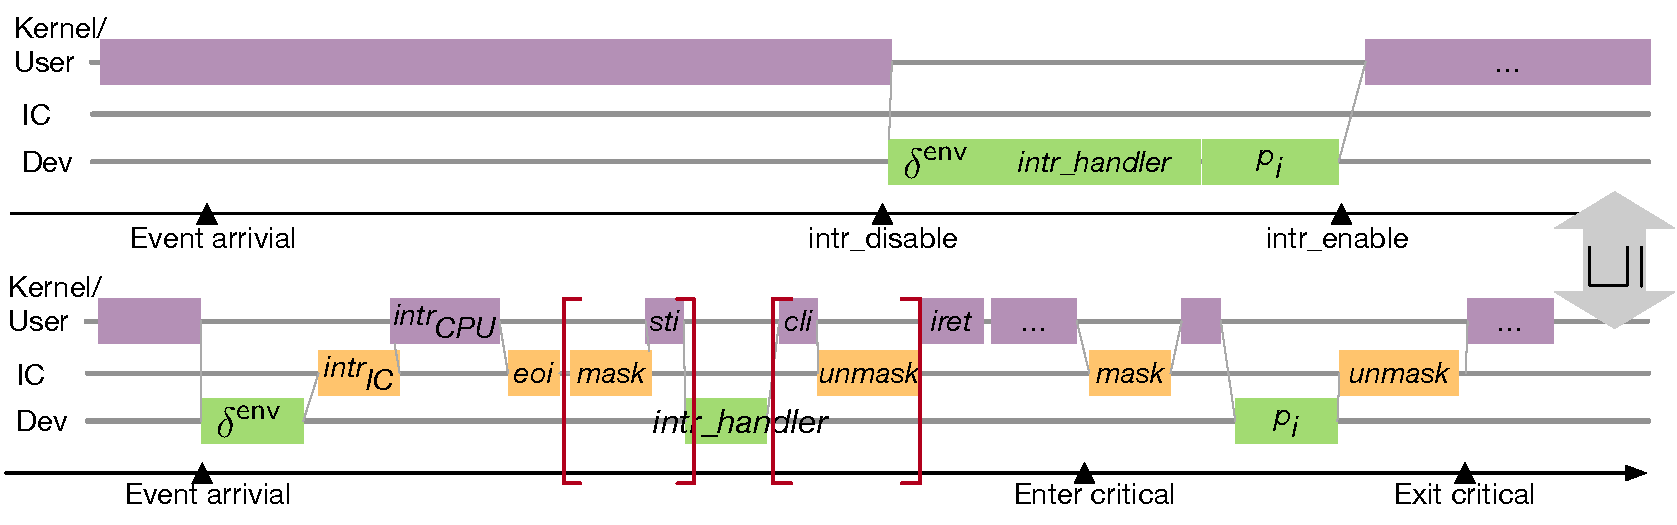
\includegraphics[width=0.95\textwidth]{figs/interrupt_nest}
	\end{center}
	\caption{The contextual refinement between interrupt models with nested interrupts.}
	\label{fig:intr_enable_nested}
\end{figure}


At this abstract interrupt model, every access to the device's abstract
states needs to be guarded by a call to {\it intr\_disable}, and this
is systematically enforced through explicit preconditions of all device primitives. 
Note that at this level, an interrupt handler of a device only changes
abstract states of that particular device. Thus, the correctness of
deferring handling all the interrupts to {\it intr\_disable} and {\it intr\_enable}
naturally follows, as none of the ``non-critical'' steps outside the pair
can change the states of the device, nor reading any states of the device.


\subsubsection{Nested Interrupts}

Note that the $\texttt{intr}_{\textsf{CPU}}$ transition in
Fig.~\ref{fig:interrupt-cpu} disables the interrupt. Thus between
$\texttt{intr}_{\textsf{CPU}}$ and $\texttt{iret}$ in
Fig.~\ref{fig:int-whole-system}, the interrupt is turned off, which means that
no nested interrupts are allowed. In many cases, supporting nested interrupts is
critical so that some high priority interrupt processing is not delayed by the
low priority ones.  The interrupt transition for the whole system with nested
interrupts is shown in Fig.~\ref{fig:int-whole-system-nested}.  Here, before the
interrupt handler is called, we mask the interrupt line of the particular device
(to make sure there is no nested interrupt from the same device) and then turn
on the interrupt on the CPU. Accordingly, after the interrupt handling, we
disable the CPU interrupt, then unmask the particular interrupt line before the
$\texttt{iret}$ transition is performed.  We have proved that this model also
refines the same abstract interrupt model (see
Fig.~\ref{fig:intr_enable_nested}).

\ignore{
\begin{lemma}
	IRQs do not affect the kernel\footnote{Remember, we consider device drivers 
	a part of the device, not the kernel.}.
\end{lemma}
\begin{myproof}
	The proof can be done through case analysis. 
	\begin{itemize}	
	\item If the particular interrupt line is masked in the IC, the CPU does not
	receive the interrupt request.

	\item If the interrupt line is not masked, but interrupts are disabled on 
	the	CPU, the interrupt signal is ignored.

	\item If the interrupt line is not masked and interrupts are enabled, the 
	CPU receives the interrupt signal and performs its own {\it intr} 
	transition. The state transition of the whole system is shown in
        Fig.~\ref{fig:int-whole-system}.
        Thus, it is sufficient to show that $d'' = d$, 
	$m'' = m$, and $\rho'' = \rho$. These can be proven by composing the 
	{\it intr} and {\it iret} with Lemma \ref{lemma:context}.
		

\end{itemize}

\end{myproof}


\begin{lemma}
An IRQ is transparent to the IC. 
\end{lemma}
\begin{myproof}
If the particular interrupt line is masked, the IC ignores the interrupt.
Otherwise, the IC does its {\it intr} transition, and the signal goes to
the CPU. If interrupts are enabled in that CPU, then CPU performs the relevant
transition, otherwise, if the interrupt is disabled, the interrupt eventually 
gets handled by the CPU when the CPU enables the interrupt through {\it sti}. 
In either case, the {\it eoi} primitive in IC is called (see
Fig.~\ref{fig:int-whole-system}).\footnote{If the CPU never re-enables another 
interrupt, its correctness is independent of what interrupt gets triggered.}
\end{myproof}
}

%\asectskip

